\section{What we have done within recent weeks}

Totally we have 10 meetings within 3 weeks. We had our first meeting to get to know each other and finalise on group name and team coordinator. All members registered on the GitHub and completed initial tasks as set by Dr.Tratt. In our second meeting, we analysed what our tasks are and distributed research tasks on server, unit tests, mobile/desktop dev, file sync and conflict resolution algorithm amongst team members. \\\\
The following meeting, some decisions on the technology to be used were made. In this meeting, we moved from Amazon EC2 to S3. \\\\
In the following meetings, we started working on our desktop application as well as the initial report. Sections of the report was allocated to each member who worked individually and pushed to git. The team co-ordinator then made some overall refactoring for the final report. Also, Lili Chen designed a sample user interface of the desktop application using MockingBot. \\\

\begin{figure}[H]
\centering
\includegraphics[scale=0.11]{desktop-ui}
\caption{Mock UI for desktop client}
\end{figure}

\begin{sidewaysfigure}
\centering
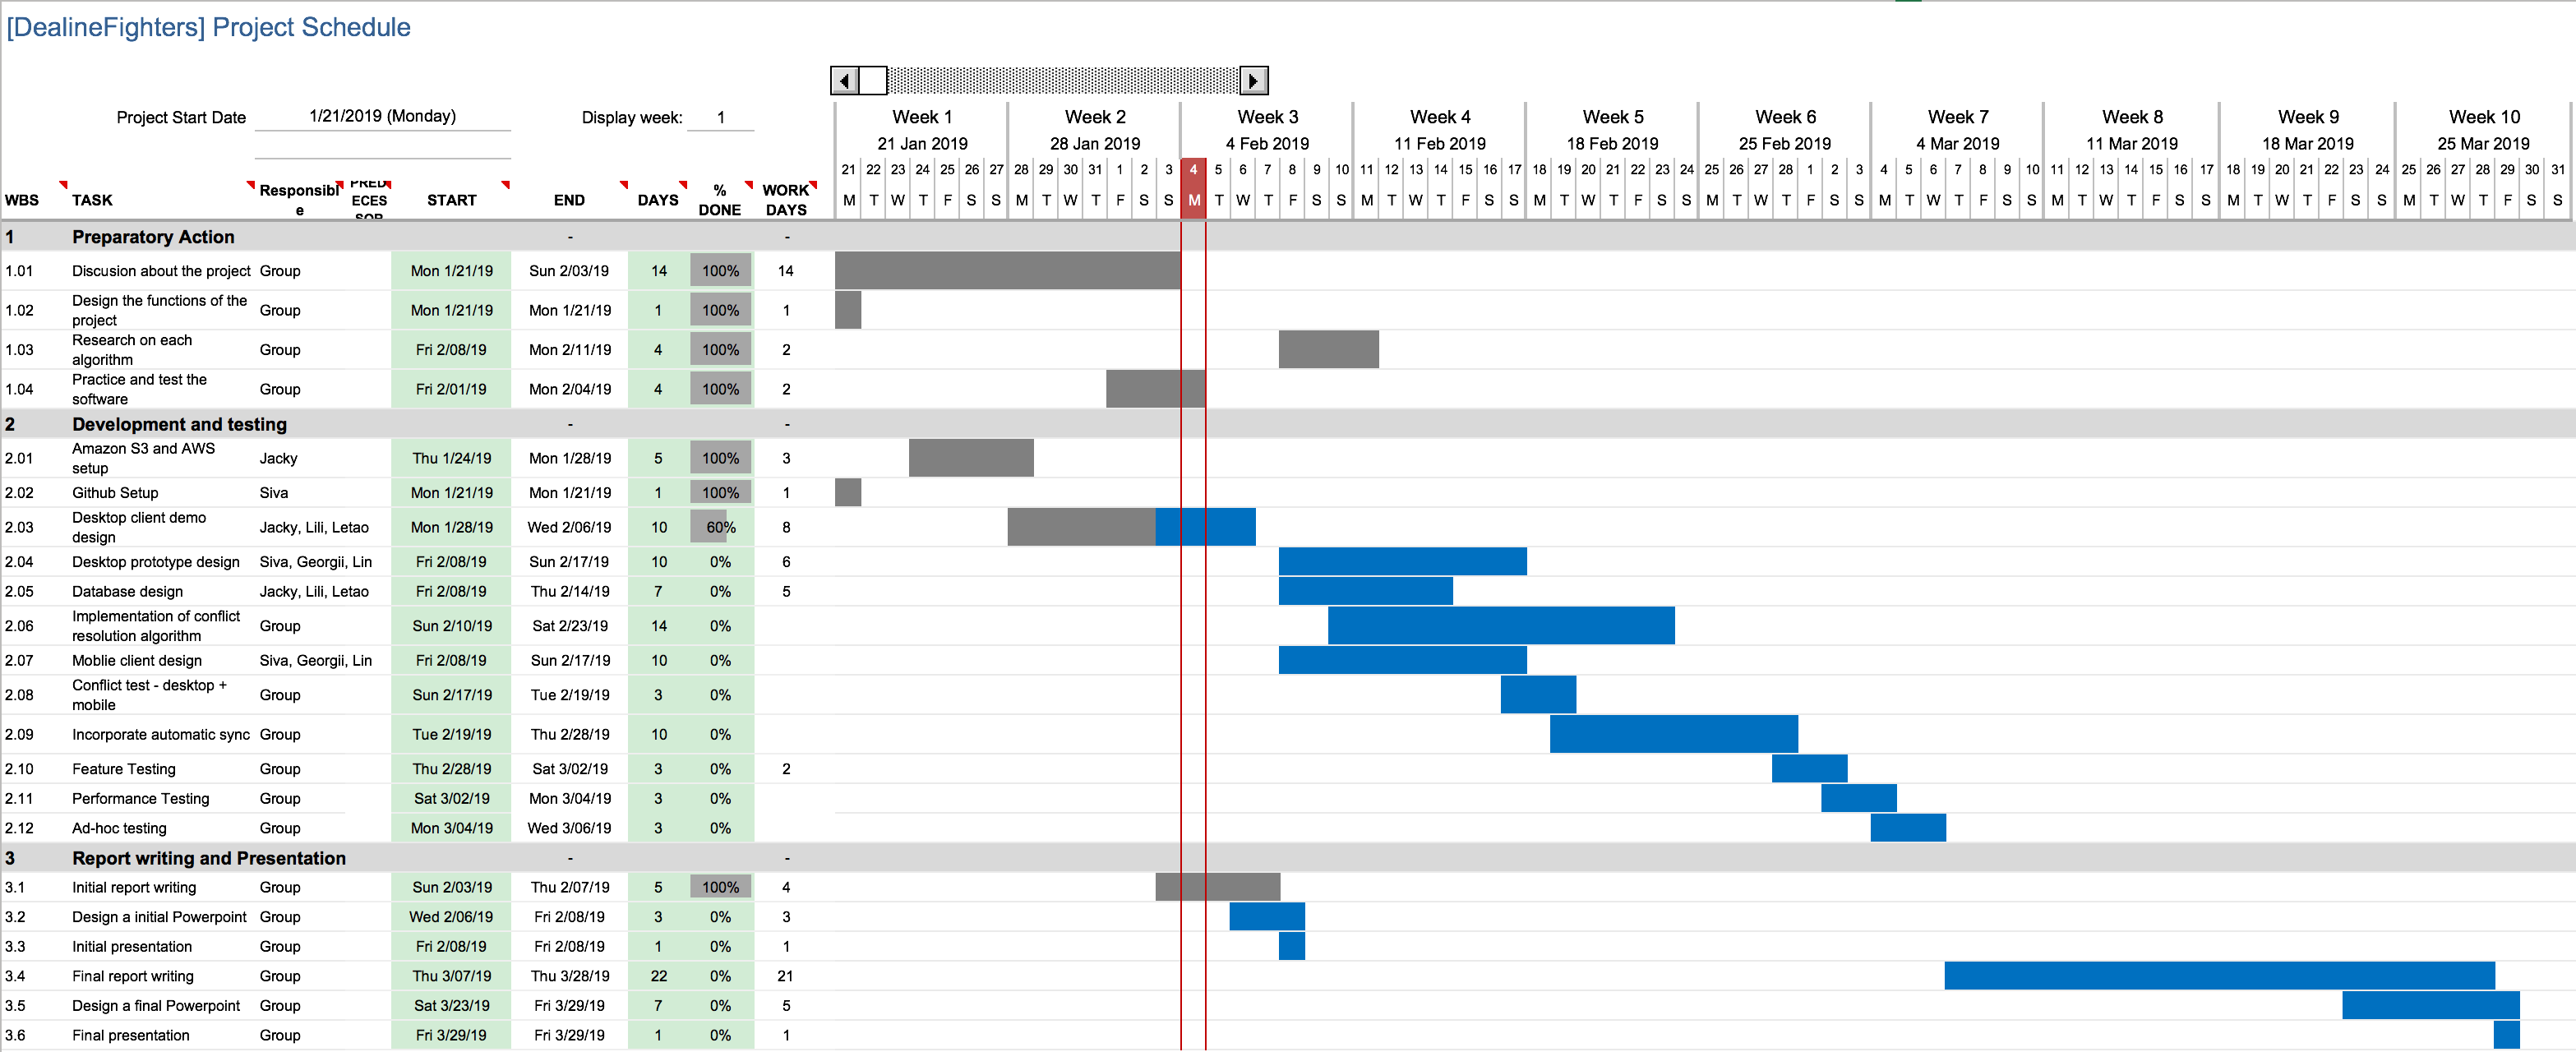
\includegraphics[scale=0.5]{Timeline_Ver_0}
\caption{This is Gantt chart which illustrates the plan of our group within 10 weeks.}
\end{sidewaysfigure}\newpage
